\chapter{Streaming}
\label{chapter:streaming}

When rendering a BTF in a web-browser the data has to be transferred before the rendering can start on a client side.
Even  compressed BTF data of size 10-20 Mb will take time for full transmission.
Assume an average user, with a 8Mbit/s connection speed.
Depending on the internet connection speed of a user, the full transmission of hight quality BTF could take several minutes.
 The solution to skip this waiting time, we propose to use progressive streaming of BTF data.
Implementing a streaming technique a user will be able to see a low quality preview of original BTF just in a few seconds. 
In our case, principal components that cover full angular domain will be streamed one by one using WebSockets \cite{websockets}.
The rendering will be refreshed whenever a new component arrives.
With each new component the quality of rendering will be progressively improved.
 Also, it is possible to show an overall progress for an user, which makes the process of streaming even more interactive.
\subsection{Web Sockets}
\label{chapter:sockets}

We use WebSockets for streaming the data, as it is most efficient and elegant way of communicating between a server and a client.
The following advantages of WebSocket technology \cite[Ch.\ 1]{websockets}:

\begin{itemize}
  \item \textbf{Delivers high \emph{Performace}}  for real-time server-client connections. 
  Usually, web developers used well known methods such as polling, long polling, and HTTP streaming. However, WebSocket saves bandwidth, CPU power, and latency compared to those methods.
  For example, polling method makes requests to the server and has to wait for the response.
  With WebSockets the client does not need to wait for the response, because WebSockets reuse the same connection from client to the server and wise-verse.
  This single connection reduces the latency.

  \item \textbf{\emph{Saves time}} to develop web-applications. \emph{Simplicity} of is one of the main advantage over older methods for server-client communication.
  
\end{itemize}

\begin{figure}[h]
 \centering
 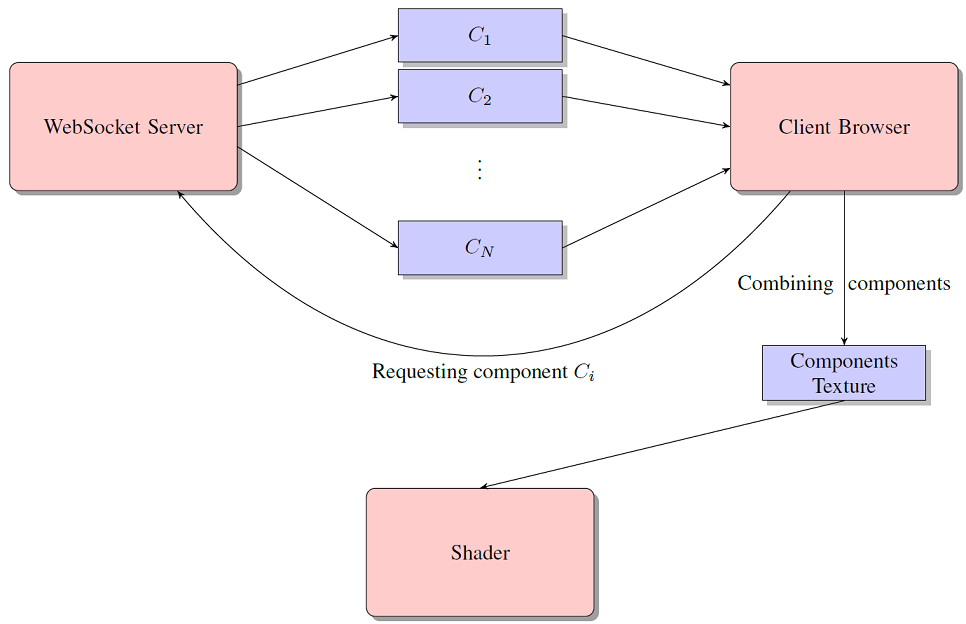
\includegraphics[width=1.0\textwidth]{figures/streaming}
 \caption[Streaming process illustration ] {
 	{\bf Streaming process illustration}
	}
 \label{fig:streaming}
\end{figure}


As it was described in Section \ref{section:algorithm_step} matrices $U$, $\Sigma$ and $V$ store all needed data to reconstruct BTF.
Matrices $\Sigma$ and $V$ are quite small in size, they are sent at first place. On the contrary, matrix $U$ stores principal components of size $W \times H$ which makes matrix $U$ the biggest in size of all.
On a client side before streaming, matrix $U$ is initialized with blank values, for example zeros. After a Socket connection was established, the client side requests one component at a time. 
Each new arrived component saved in matrix $U$ and the client side refreshes the shader to render BTF. Figure \ref{fig:streaming} illustrates this process.
 Also, each component is saved as PNG image on the WebSocket server, which makes a bit further compression of the BTF.

Consider Figure \ref{fig:streamPreview} that shows how the streaming works on practice.
We can see that even with first components the resulted texture looks quite decent.
With further components the overall quality of texture improves, e.g. specularities are increasing, small micro-structures become more visible and emphasized.
To make the streaming process a bit entertaining, the client also can see the progress-bar of the streaming progress.
Also, some of the mid-results were skipped in the Figure \ref{fig:streamPreview} for the sake of simplicity.

\begin{figure}[h]
 \centering
 \includegraphics[width=1.0\textwidth]{figures/streampreview}
 \caption[Example of Progressive Streaming ] {
 	{\bf Example of Progressive Streaming}

	\textbf{From left to right}: \emph{1}, \emph{2}, \emph{4}, \emph{6}, \emph{7}  components rendered at the same time.
	
	\textbf{Note}: \emph{8th} component is average grey value, which sends at first place.
	}
 \label{fig:streamPreview}
\end{figure}

\subsection{Transmission}
\label{chapter:transmission}
